\part{Parallelism}

The simplicity of the Transformers architecture lends itself to a deep variety of parallelism
strategies. We review some of them below.

\subsection{Tensor Parallelism \label{subsec_tensor_parallelism} }

\begin{commentbox}{Side Note: }
    I wrote a blog post on this \href{https://www.determined.ai/blog/tp}{here.}
\end{commentbox}


In \textbf{Tensor Parallelism}, sometimes also called \textbf{Model Parallelism}, individual weight
matrices are split across devices \cite{shoeybi2020megatronlm}. We consider the \pyinline{MLP} and
\pyinline{CausalAttention} layers in turn. Assume $ T $-way parallelism such that we split some
hidden dimension into $ T $-equal parts across $ T $ workers\footnote{All $ T $ workers work on
    processing the same batch collectively.  With $ N>T $ workers, with $ N $ perfectly divisible by
    $ T $, there are $ N/T $ different data parallel groups. Critical-path TP communications occur
    within each data parallel group and gradients are synced across groups. Ideally, all the workers
    in a group reside on the same node, hence the usual $ T=8 $.}


\begin{nicebox}{Essentials}
	The cost of large weights can be amortized by first sharding its output dimension, resulting in
	differing activations across group members. Later, the activations are brought back in sync via
	a \pyinline{AllReduce}. Weights which act on the sharded-activations can also be sharded in their
	input dimension. In the backwards pass, another \pyinline{AllReduce} is required.
\end{nicebox}

\paragraph{MLP}
It is straightforward to find the reasonable ways in which the weights can be partitioned. We
suppress all indices apart from those of the hidden dimension for clarity.

The first matrix multiply $ z _{ d }W ^{ 0 } _{ d e } $ is naturally partitioned across the output
index, which spans the expanded hidden dimension $ e\in \left \{ 0, \ldots , ED-1 \right \} $. This
functions by splitting the weight matrix across its output indices across $ T $ devices:  $ W ^{ 0 }
_{ d e }= W ^{ 0 }_{ d (f t) } \equiv  \bar{W} ^{ 0 } _{ d f \bar{t} }$ (again in
\pyinline{einops}-like notation, with bars denoting that the tensor and particular indices are
sharded; see App.~\ref{app_conventions}), where in the split weights $ \bar{t}\in \left \{ 0, \ldots
, T-1 \right \} $, and $ f \in \left \{ 0, \ldots , \frac{ ED }{ T } -1\right \} $. Each of the $ T
$ workers compute one shard of $ z _{ d }\bar{W} ^{ 0 }_{ df \bar{t} } $, i.e. each has a different
value of $ \bar{t} $.


Let the partial outputs from the previous step be $ \bar{z} _{ ft }  $ (batch-index suppressed),
which are \pyinline{(B, S, E*D/T, T)}-shaped, with the final dimension sharded across workers. The
non-linearity $ \phi $ acts element wise, and using the updated $ \bar{z} _{ f \bar{t} }   $ to
compute the second matrix multiply requires a splitting the weights as in $ W ^{ 1 } _{ e d' }= W ^{
1 }_{ (ft)d' } \equiv \bar{W} ^{ 1 } _{  f \bar{t} d'}$ (dividing up the incoming $ e $ dimension),
such that the desired output is computed as in $  \bar{z} _{ f \bar{t} }\cdot \bar{W} ^{ 1 }_{ f
\bar{t}d' }$, sum over $ \bar{t} $ implied. Each device has only $\bar{t} $ component in the sum (a
\pyinline{(B, S, D)}-shaped tensor) and an \pyinline{AllReduce} is used to give all workers the
final result. This \pyinline{AllReduce} is the only forward-pass collective
communication\footnote{The amount of communicated data is $ \Ocal \left( BSD \right)$.}.

One-line summary of the parallel decomposition:
\begin{align}
 z _{ sd' } \leftarrow   \phi \left (z _{ d }W ^{ 0 }_{ de }\right )W ^{ 1 } _{ ed' } &=\phi \left (z _{ d }\bar{W} ^{ 0 }_{ df \bar{t} }\right )\bar{W} ^{ 1 } _{ f \bar{t}d' } \ .
\end{align}
The progression of tensor shapes held by any single worker is
\begin{enumerate}
    \item \pyinline{(B, S, D)}
    \item \pyinline{(B, S, E*D/T)}
    \item \pyinline {(B, S, D)}
\end{enumerate}

In the backwards pass, another \pyinline{AllReduce} (see App.~\ref{app_collective_communications})
is needed for proper gradient computations with respect to the first \pyinline{Linear} layer's
outputs. This is true whenever an operation producing a sharded output involved non-sharded tensors:
if an operation $ \bar{y}_{ \bar{r} }  = F(x, \ldots) $ produces a sharded output from an unsharded
in put $ x $ (all other indices suppressed), the derivative with respect to $ x $ requires a sum
over ranks, $ \frac{ \partial \Lcal }{ \partial x } = \frac{ \partial \Lcal }{ \partial \bar{y} _{
\bar{r} }  } \frac{ \partial \bar{y} _{ \bar{y} } }{ \partial x  }$. Note that each worker will have
to store all components of the input $ z $ for the backward pass.



\begin{figure}[ht]
	\centering
	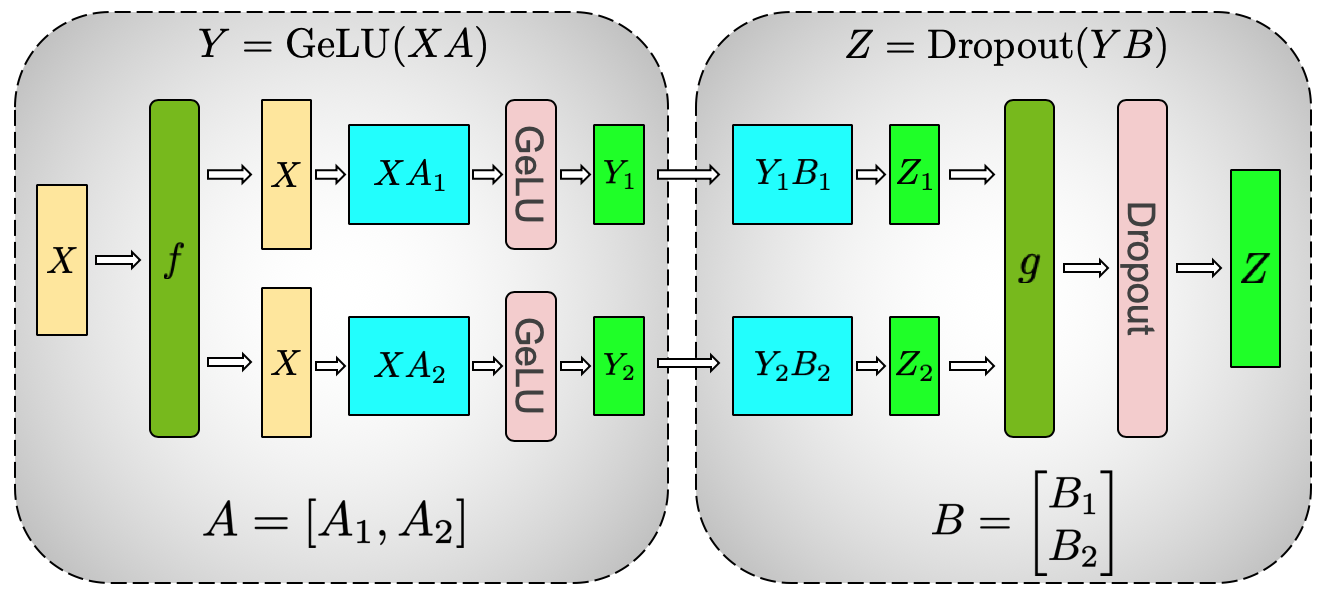
\includegraphics[scale=.33]{figures/mlp_mp_2.png}
	\caption{Tensor parallelism for the \pyinline{MLP} layers. Graphic from
		\cite{shoeybi2020megatronlm}. The $ f/g $ operations are the collective
		identity/\pyinline{AllReduce} operations in the forwards pass and the \pyinline{AllReduce}/identity
		operations in the backwards pass.}
	\label{fig_mlp_tensor_parallel}
\end{figure}


\paragraph{Attention} Because the individual attention head computations are independent, they can
be partitioned across $ T $ workers without collectively communications.  An \pyinline{AllReduce} is
needed for the final projection, however, which results in the various re-weighted values $ y _{
bsea } $ \eqref{eq_reweighted_values}.

To review, the attention outputs $ z' _{ sd } $ generated from inputs $ z_{ sd } $ can be expressed
as
\begin{align}
    z' _{ sea }  &= {\rm  MHA}(q _{ sea }, k _{ sea }, v _{ sea }) O _{ ead }\nn
\end{align}
where:
\begin{itemize}
    \item  We have split the $ d $-index as in $ z _{ sd }\longrightarrow z _{ s (ea) } $ with $ e $ and
$ a $ the head-dimension and head-index
    \item $ q _{ sea }, k _{ sea }, v _{ sea }
$ are the query, keys and values derived from the inputs
    \item ${\rm
    MHA } $ is the multi-head attention function, whose outputs are the same shape as its value inputs
    \item The dual sum over head-dimension index ($ e $) and attention-head-index ($ a $) is the
    sum-and-concatenate step from the more explicit description in Sec.~\ref{subsubsec_attn_layer}
    \item \pyinline{Dropout} and biases were ignored for simplicity
\end{itemize}

In order to parallelize the above $ T $-ways, we simply shard across the dimension $ a $  which
indexes the different attention heads.  The $ {\rm MHA} $ computations all process in
embarassingly-parallel fashion, and an all-reduce is needed to complete the sum over the $ a $-index
across devices.

The collective communications story is essentially
equivalent to that of the \pyinline{MLP} layers\footnote{The amount of communicated data is again $ \Ocal \left( BSD
\right)$. }: one \pyinline{AllReduce} is needed in the forwards pass
and one \pyinline{AllReduce} in the backwards-pass.

The progression of tensor shapes held by any single worker is
\begin{enumerate}
    \item \pyinline{(B, S, D)}
    \item \pyinline{(B, S, D/A, A/T)}
    \item \pyinline {(B, S, D)}
\end{enumerate}


It is worth comparing the communications and FLOPs costs of these sharded layers. Each layer costs
$ \Ocal \left(    BS \left ( 4+2E \right )  D ^{ 2 }/T \right)$ FLOPs and communicates
$ \Ocal \left( BSD \right)  $ bytes and so the communication-to-compute-time ratio is
\begin{align}
  \frac{ t _{ {\rm  compute} } }{ t _{ {\rm  comms} } } & \sim  \frac{ \left ( 4+2E \right) D }{ T }\times \frac{ \lambda _{ {\rm comms} }  }{ \lambda _{ {\rm FLOP/s} }} \ .
\end{align}
Since\footnote{Assuming $ \lambda _{\rm  FLOP/s }\sim  $100 TFLOP/s and $ \lambda _{ {\rm comms} }
\sim $ 100 GiB/s.} $ \frac{ \lambda _{ {\rm comms} }  }{ \lambda _{ {\rm FLOP/s} }} \sim 10 ^{ -3 }
$FLOPs/B, communication and compute take similar times when  $ D \sim \Ocal \left( 10 ^{ 3 } \right)
$ for typical setups with $ T \sim \Ocal \left( 10 \right)  $ and so tensor-parallelism requires
$ D \gtrsim 10 ^{ 4 } $ to reach similar efficiency to the non-tensor-parallel implementations.


\begin{figure}[ht]
	\centering
	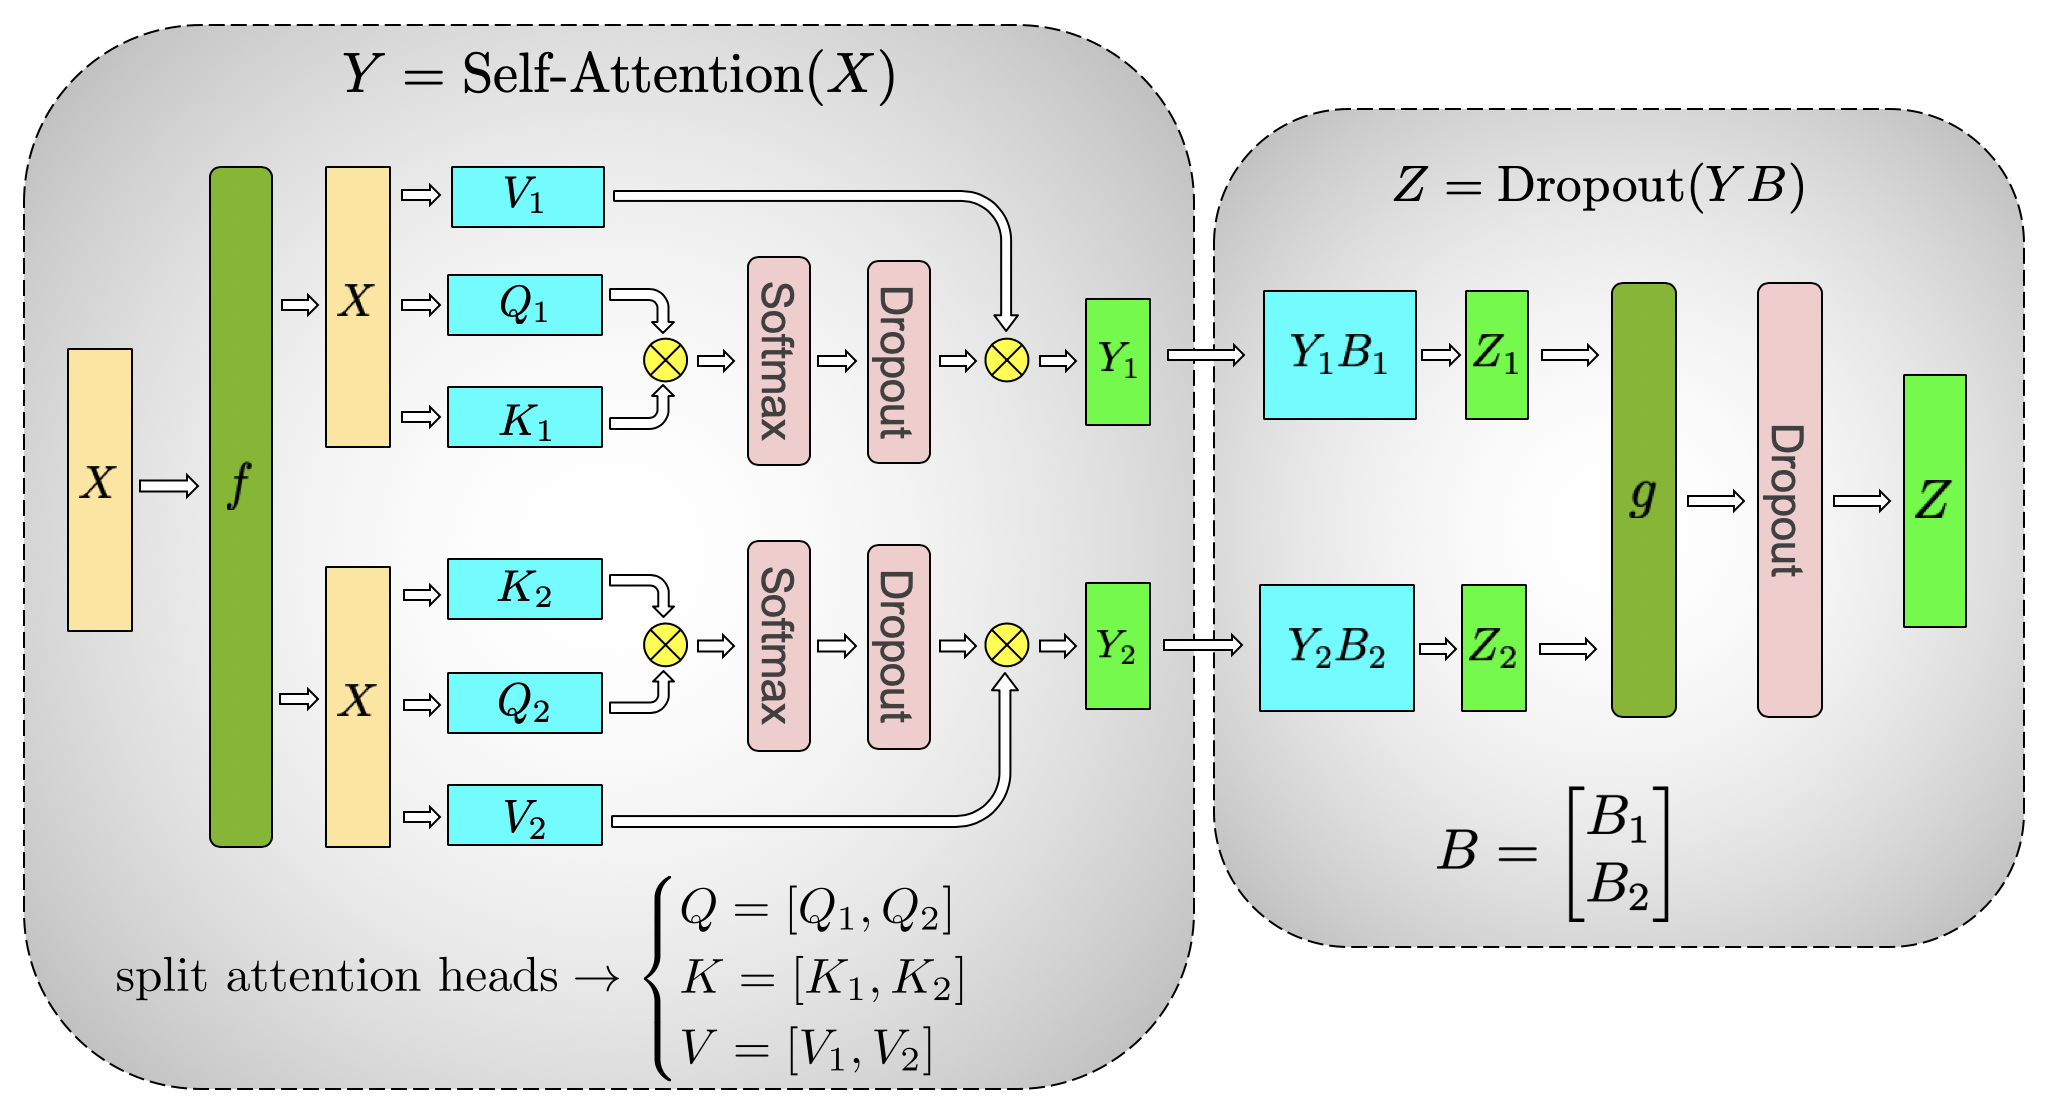
\includegraphics[scale=.45]{figures/attention_mp_2.png}
	\caption{Tensor parallelism for the \pyinline{CausalAttention} layers. Graphic from
		\cite{shoeybi2020megatronlm}. The $ f/g $ operators play the same role as in
		Fig.~\ref{fig_mlp_tensor_parallel}.}
	\label{fig_attn_tensor_parallel}
\end{figure}

\paragraph{Embedding and LM Head} Last, we can apply tensor parallelism to the language model head,
which will also necessitate sharding the embedding layer, if the two share weights, as typical.

For the LM head, we shard the output dimension as should be now familiar, ending up with $ T $
different \pyinline{(B, S, V/T)}-shaped tensors, one per group member. Rather than communicating
these large tensors around and then computing the cross-entropy loss, it is more efficient to have
each worker compute their own loss where possible and then communicate the scalar losses
around\footnote{In more detail, given the gold-answers $ y _{ bs } $ for the next-token-targets, a
	given worker can compute their contribution to the loss whenever their \pyinline{(B, S, V/T)}-shaped
	output $ z _{ bsv' } $ contains the vocabulary dimension $ v _{ * } $ specified by $ y _{ bs } $,
	otherwise those tensor components are ignored.}.

For a weight-tied embedding layer, the former construction requires \pyinline{AllReduce} in order
for every worker to get the full continuous representation of the input.

\paragraph{LayerNorm and Dropout} \pyinline{LayerNorm} instances are not sharded in pure tensor
parallelism both because there is less gain in sharding them parameter-wise, but also sharding
\pyinline{LayerNorm} in particular would require additional cross-worker communication, which we
wish to reduce as much as possible. \pyinline{Dropout} layers are also not sharded in  where
possible in pure tensor parallelism, but sharding the post-attention \pyinline{Dropout} layer is
unavoidable. It is the goal of sequence parallelism is to shard these layers efficiently; see
Sec.~\ref{subsec_seq_parallelism}.

\paragraph{Effects on Memory} The per-worker memory savings come from the sharding of the weights
and the reduced activation memory from sharded intermediate representations.

The gradient and optimizer state memory cost is proportional to the number of parameters local to
each worker (later we will also consider sharding these components to reduce redundantly-held
information). The number of parameters per worker is reduced to
\begin{align}
	N _{ \rm params } & \approx  (4 + 2E) \frac{ L D ^{ 2 } }{ T }\ ,
	\label{eq_approx_params_tensor_parallel}
\end{align}
counting only the dominant contribution from weights which scale with $ L $, since every weight is
sharded. Since all non-activation contributions to training memory scale with $ N _{ {\rm params}  }
$, this is a pure $ 1/T $ improvement.

The per-layer activation memory costs \eqref{eq_att_actmem_vanilla} and
\eqref{eq_mlp_actmem_vanilla} are altered to:
\begin{align}
	M _{ \rm act  } ^\texttt{Attention} & = BS \left ( \left (p + \frac{ 4p }{ T }+1 \right )D + \left
		(\frac{ 2p+1 }{ T } \right )AS  \right ) \nn
	M _{ \rm act  } ^\texttt{MLP}       & = \left (\frac{ 2Ep }{ T }+p+1 \right )BDS\ .
	\label{eq_act_mem_attn_mlp}
\end{align}
The derivation is similar to before. Adding in the (unchanged) contributions from
\pyinline{LayerNorm} instances, the total, leading order activation memory sums to
\begin{align}
	M _{ {\rm act}  } ^{ {\rm  total}  } & \approx  2BDLS   \left ( p \left (2+ \frac{ E+2 }{ T }\right ) + 1   \right )
	+ ABLS ^{ 2 } \left ( \frac{ 2p+1 }{ T }\right ) \label{eq_act_mem_total_tensor_parallel}\ .
\end{align}
Again, the terms which did not receive the $ 1/T $ enhancement correspond to activations from
unsharded \pyinline{LayerNorm} and \pyinline{Dropout} instances and the $ 1/T $'s improvements can
be enacted by layering sequence parallelism on top (Sec.~\ref{subsec_seq_parallelism}).


\subsection{Sequence Parallelism \label{subsec_seq_parallelism}}

In \eqref{eq_act_mem_total_tensor_parallel}, not every factor is reduced by $ T $. \textbf{Sequence
	Parallelism} fixes that by noting that the remaining contributions, which essentially come from
\pyinline{Dropout} and \pyinline{LayerNorm}\footnote{Recall, though, from
	Sec.~\ref{subsubsec_layer_norm} that the parameters in \pyinline{LayerNorm} are completely redundant
	and can simply be removed without having any effect on the expressive capabilities of the
	architecture.}, can be parallelized in the sequence dimension (as can the residual connections).

The collective communications change a bit. If we shard the tensors across the sequence dimension
before the first \pyinline{LayerNorm}, then we want the following:
\begin{enumerate}
	\item The sequence dimension must be restored for the \pyinline{CausalAttention} layer
	\item The sequence should be re-split along the sequence dimension for the next \pyinline{LayerNorm} instance
	\item The sequence dimension should be restored for the \pyinline{MLP} layer \footnote{This doesn't
		      seem like a hard-requirement, but it's what is done in \cite{korthikanti2022reducing}.}
\end{enumerate}

The easiest way to achieve the above is the following.
\begin{enumerate}
	\item If the tensor parallelization degree is $ T $, we also use sequence parallelization degree $ T
	      $.
	\item The outputs of the first \pyinline{LayerNorm} are \pyinline{AllGather}-ed to form the full-dimension
	      inputs to the \pyinline{CausalAttention}  layer
	\item The tensor-parallel \pyinline{CausalAttention} layer functions much like in
	      Fig.~\ref{fig_attn_tensor_parallel} \textit{except} that we do not re-form the outputs to
	      full-dimensionality.  Instead, before the \pyinline{Dropout} layer, we \pyinline{ReduceScatter} them
	      from being hidden-sharded to sequence-sharded and pass them through the subsequent
	      \pyinline{Dropout}/\pyinline{LayerNorm} combination, similar to the first step
	\item The now-sequence-sharded tensors are reformed with another \pyinline{AllGather} to be the full-dimensionality inputs to the
	      \pyinline{MLP} layer whose final outputs are similarly \pyinline{ReduceScatter}-ed to be
	      sequence-sharded and are recombined with the residual stream
\end{enumerate}
The above allows the \pyinline{Dropout} mask and \pyinline{LayerNorm} weights to be sharded $ T
$-ways, but if we save the full inputs to the \pyinline{CausalAttention} and \pyinline{MLP}  layers
for the backwards pass, their contributions to the activation memory are not reduced (the $ p
$-dependent terms in \eqref{eq_act_mem_attn_mlp}). In \cite{korthikanti2022reducing}, they solve
this by only saving a $ 1/T $ shard of these inputs on each device during the forward pass and then
performing an extra \pyinline{AllGather} when needed during the backwards pass. Schematics can be
sen in Fig.~\ref{fig_tensor_seq_parallel} and Fig.~\ref{fig_tensor_seq_parallel_detail} below. The
activation memory is then reduced to:
\begin{align}
	M _{ {\rm act}  } ^{ {\rm  total}  } & =\frac{ 2BDLS   \left ( p(E+4) + 1   \right ) }{ T }
	+ \frac{ ABLS ^{ 2 } \left ( 2p+1\right ) }{ T }  + \Ocal \left( BSV \right) \label{eq_act_mem_total_seq_parallel}\ .
\end{align}

In more detail:
\begin{itemize}
    \item The norms are just linear operations on the $ z _{ sd }  $, $ z' _{ sd } =
{\rm Norm}\left ( z _{ sd } \right ) $, and so we split and shard cross the sequence dimension $ z
_{ sd } \longrightarrow  z _{ (tr) d }  \equiv  \bar{z}_{ \bar{t}rd }$ with the TP-index $ t $
sharded across devices.
\item The residual stream is also sharded across the sequence dimension.
\item The sharded outputs $ \bar{z}_{ \bar{t}rd } $ must be re-formed to create the
attention and MLP inputs via an \pyinline{AllGather}. There is an optimization choice here:
either the re-formed tensors can be saved for the backward pass (negating the $ 1/T $ memory
savings) or they can be re-formed via an \pyinline{AllGather}, at the cost of extra communication.
\item Both the MLP and attention layers need to produce final sums of the form $ \bar{y} _{ s
    \bar{y} e } \bar{O} _{ \bar{t} ed } $ for some intermediate $ \bar{y} $ and weight $ \bar{O} $
    sharded across the TP-dimension $ \bar{t} $. The outputs are added to the sequence-sharded residual
    stream, and so sum is optimally computed through an \pyinline{ReduceScatter} with final shape $
    \bar{z} _{ \bar{t}'rd } = z _{ (t'r)d } = z _{  sd } =\bar{y} _{ s \bar{t} e } \bar{O} _{ \bar{t}
    ed } $. This \pyinline{ReduceScatter} (along with the \pyinline{AllGather} mentioned above)
    replace the \pyinline{AllReduce}s from the tensor-parallel case and have the same overall
    communication cost.
\end{itemize}


\begin{figure}[ht]
	\centering
	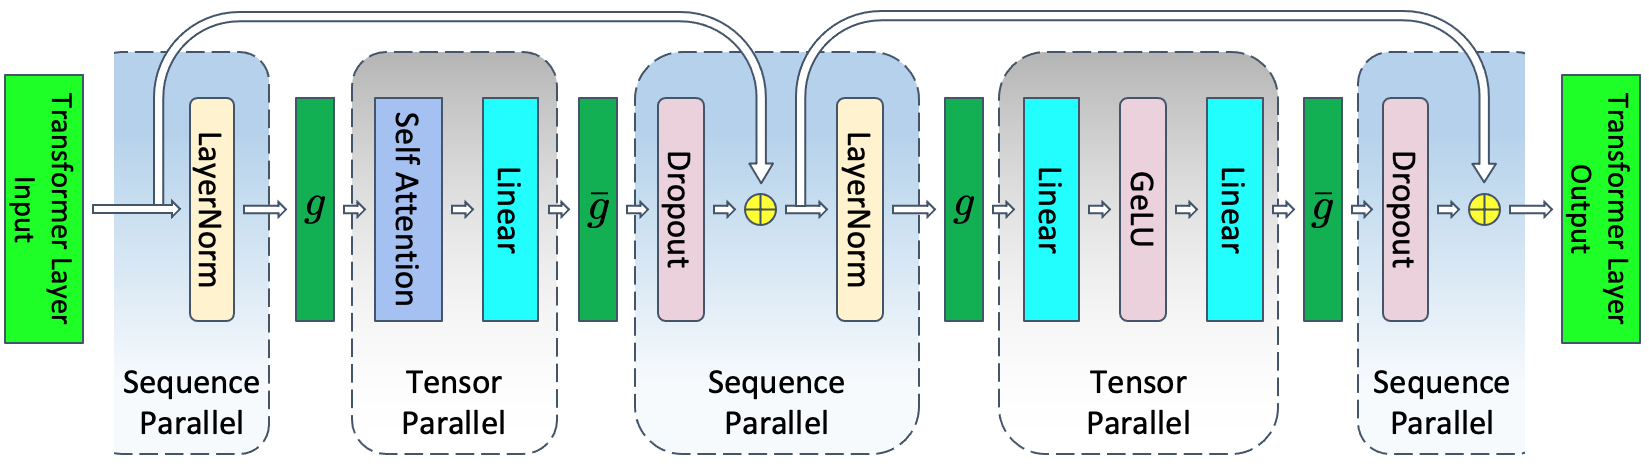
\includegraphics[scale=.25]{figures/transformer-tensor-sequence-parallel.jpg}
    \caption{Interleaved sequence and tensor parallel sections. $ g $ and $ \bar{g} $ are
    \pyinline{AllGather} and  \pyinline{ReduceScatter} in the forward pass, respectively, and swap
roles in the backwards pass. Graphic from \cite{shoeybi2020megatronlm}. }
	\label{fig_tensor_seq_parallel}
\end{figure}

\begin{figure}[ht]
	\centering
	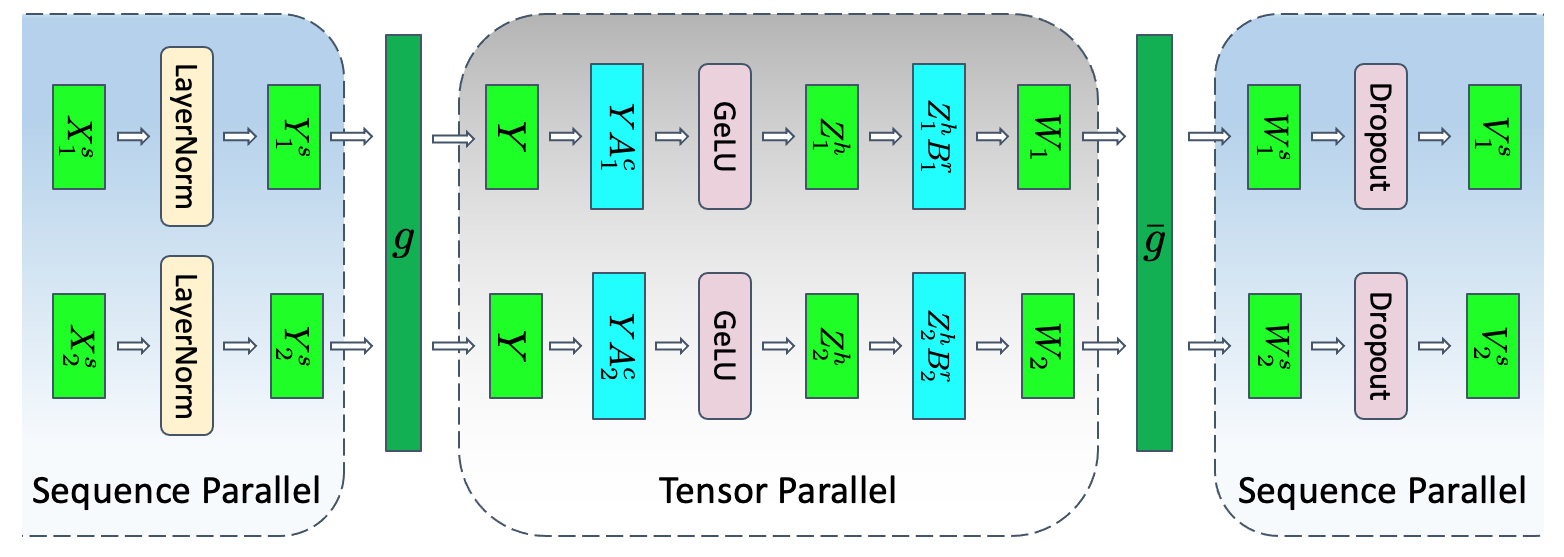
\includegraphics[scale=.25]{figures/mlp-tensor-sequence-parallel.jpg}
	\caption{Detail of the sequence-tensor parallel transition for the \pyinline{MLP} . Graphic from
		\cite{shoeybi2020megatronlm}. }
	\label{fig_tensor_seq_parallel_detail}
\end{figure}


\subsection{Ring Attention \label{subsec_ring_attention}}

Ring Attention \cite{liu2023ringattentionblockwisetransformers} is roughly a distributed version of
Flash Attention \ref{subsec_flash_attention}: it enables extremely long sequence-length processing
by never realizing the entire $ \Ocal \left( S ^{ 2 } \right)  $ attention scores at once.

It works by sharding over the sequence dimension. Let $ z _{ sd } $ is the (batch-dim suppressed)
residual stream of a non-sharded Transformer:
\begin{align}
    z _{  sd } &= \Sm _{ s' } \left ( q _{ sd' } k _{ s'd' } /\sqrt{D}\right ) v _{ s'd } \ ,
\end{align}
suppressing the causal mask for simplicity of presentation.

Then in Ring Attention, we shard over $ R $ devices via $ z _{ sd } \longrightarrow z _{ \bar{r}td }
$, and similar for other tensors, to compute the sharded outputs
\begin{align}
    z _{  \bar{r}td } &= \Sm _{ \bar{w} x  } \left ( q _{ \bar{r}t d' } k _{ \bar{w}x d' } \right ) v _{ \bar{w}x d }\nn
     &= \frac{ \exp \left ( q _{ \bar{r}t d' } k _{ \bar{w}x d' }/\sqrt{D} \right ) }{ \sum _{ \bar{w}'x' } \exp \left (q _{ \bar{r}t d'' } k _{ \bar{w}'x' d'' }/\sqrt{D}\right )  } v _{ \bar{w}xd }\nn
     &\equiv \frac{ Z _{\bar{r}td } }{   \sum _{ \bar{w}'x' } \exp  \left (q _{ \bar{r}t d'' } k _{ \bar{w}'x' d'' }/\sqrt{D} \right ) }\nn
     &\equiv \frac{ Z _{\bar{r}td } }{L _{ \bar{r}t }}
\end{align}
where we introduced some notation which will be useful blow. Ring Attention is essentially an
algorithm for computing the sharded sums over barred indices via communication. Since the MLP layers
act on every sequence position identically, only the Attention layers (and the loss computation)
require special handling.

The algorithm performs the $ \bar{w}$ sum as a loop. We present the simplified case without a causal
mask or maximum attention score tracking. These are important omissions\footnote{See
\cite{brandon2023stripedattentionfasterring} for causal mask efficiency considerations.}.
\begin{algo}{Ring Attention (Naive - Missing causal mask/max tracking.)}
\State Initialize $ Z _{ \bar{r}td } $, $ L _{ \bar{r}t } $ to zeros
\State Populate the key, query, and value shards $ q _{ \bar{r}td },k _{ \bar{w}x d' },v _{ \bar{w}x d' } $ with $ \bar{r} =  \bar{w} = r $ on rank $ r $
\For{ $ w \in \left \{ r, \ldots , R-1, 0, \ldots , r-1 \right \}  $} \Comment Computing components $ z _{ \bar{r}td } $ $ \forall t, d $
    \If{$ w \neq (r-1) \mod R $} prefetch shards $ k _{ (\bar{w}+1)xd }, v _{ (\bar{w}+1)xd } $ $ \forall x,d $
    \EndIf
    \State $ Z _{ \bar{r}td } \gets Z _{ \bar{r}td }+   \exp \left ( q _{ \bar{r}t d' } k _{ \bar{w}x d' }/\sqrt{D} \right ) v _{ \bar{w}xd } $ \Comment Can use flash attention kernels here
    \State $ L _{ \bar{r}t } \gets  L _{ \bar{r}t } +  \sum _{ x } \exp \left ( q _{ \bar{r}t d' } k _{ \bar{w}x d' }/\sqrt{D}\right )  $ \Comment Can use flash attention kernels here
\EndFor
\State $ z _{ \bar{r}td } \gets \frac{ Z _{ \bar{r}td } }{ L _{ \bar{r}t }  }$
\label{algo_ring_attn_fwd_naive}
\end{algo}

At every step in the loop in the algorithm we are computing the sums $ \exp \left ( q _{ \bar{r}t d'
} k _{ \bar{w}x d' } \right ) v _{ \bar{w}xd } $ and $ \sum _{ x } \exp \left ( q _{ \bar{r}t d' } k
_{ \bar{w}x d' } \right)  $ for fixed values of $ \bar{r}, \bar{w} $ and all values of the other
indices. These are precisely the ingredients that go into the usual attention computation and for
this reason it's possible to use flash attention kernels for every individual step. \pyinline{torch}
implementations of Ring Attention which leverage flash attention kernels can be found
\href{https://github.com/lucidrains/ring-attention-pytorch}{here} and
\href{https://github.com/zhuzilin/ring-flash-attention}{here}.

The full forms of the forwards and backwards passes are again similar to those of flash attention; see Sec. \ref{subsubsec_fa_details}.

\subsubsection{The Causal Mask}

A naive, row-major sharding of the queries, keys, and vectors is highly suboptimal for causal
attention because it leads to idling GPUs. Sharding the queries and keys as in $ q _{ s } =q _{
(\bar{r}t) } $ and $ k _{ s' } = k _{ (t'\bar{r}') } $ in row-major order\footnote{That is, $ s = \bar{r}T
+ t $ for $ \bar{r} \in \left \{ 0, \ldots , R-1 \right \} $ and $ t \in \left \{ 0, \ldots  T-1
\right \} $ with $ S=RT $.}, causality means that the entire chunked attention computation will be
trivial for any iteration in which $ r'> r $. This is the case for $ R-1 $ iterations for the $ r=0
$ GPU, for instance.

So, we shouldn't shard this way for ring attention. In \cite{brandon2023stripedattentionfasterring}
they demonstrate the speed-up achieved by just reversing the sharding pattern to column-major: $ q
_{ s } =q _{ (t\bar{r}) } $ and $ k _{ s' } = k _{ (t'\bar{r}') } $ which guarantees non-trivial
work for every GPU on every iteration. In the \texttt{ring-flash-attention} repo, they come up with
yet another sharding strategy ("zig-zag" attention;
\href{https://github.com/zhuzilin/ring-flash-attention/issues/2}{see this github issue}) which
increases efficiency even more. Their strategy can't be naturally writtein in \texttt{einops}
notation, but it is easy enough to explain: they split the sequence length into $ 2R $ sequential
chunks and give zero-indexed chunks $ r $ and $ 2R -r -1 $ to GPU $ r $, which ends up guaranteeing
that at least half of the computations will be non-trivial for every GPU for every stage of the
computation.



\subsection{Pipeline Parallelism \label{subsec_pipe_parallelism}}

TODO
